\documentclass[11pt]{beamer}

%%% \mode must be on a line by its own, without comment or whitespace!
%%% \mode sets the mode to presentation. So if the mode is presentation the slides after are shown
%%% if the mode is not presentation (but article or handout) they are not shown
\mode<presentation>{}

%\usetheme{Warsaw}
\usetheme{Dresden}
%\usetheme{Copenhagen}
%\usetheme{Montpellier}
\usepackage[utf8]{inputenc}
\usepackage[english]{babel}
\usepackage{amsmath}
\usepackage{amsfonts}
\usepackage{amssymb}
\usepackage{graphicx}
\usepackage{xspace}
\usepackage{tikz}
%\usetikzlibrary{snakes} % decorations in stead of snakes
\usepackage{tikz}
\usetikzlibrary{arrows,decorations.pathmorphing,backgrounds,positioning,fit,petri}
%\usetikzlibrary{pictures}
%\usepackage{chronology} % removed: doesn't work

\author{Team33}
\title{Final Presentation\\(XMas Designer)}
%\setbeamercovered{transparent} 
%\setbeamertemplate{navigation symbols}{} 
%\logo{} 
\institute{Open University/\\Guus Bonnema, Stefan Versluys, Jeroen Kleijn} 
\date{May 20, 2015} 
\subject{ABI project XMas Designer} 

\begin{document}

\newcommand{\Noc}{\textsc{NoC}\xspace}
\newcommand{\qt}{\textsc{Qt}\xspace}
\newcommand{\qml}{\textsc{Qml}\xspace}

\begin{frame}
	\titlepage
\end{frame}

\begin{frame}
	\frametitle{Contents}
	\begin{itemize}
		\item [Guus] Introduction 
		\item [Guus] Assignment
		\item [Stefan] Process Overview
		\item [Stefan] Contribution
		\item [Stefan] Demo
		\item [Guus] Architecture
		\item [Guus] Reflection
	\end{itemize}
	
	Vragen stellen kan achteraf en tussendoor.
	
\end{frame}

\begin{frame}
	\frametitle{Introduction}
	\begin{tabular}{lp{2.5cm}p{4cm}}
	\hline
	{\bf Student} & {\bf Role}      & {\bf Dayjob}\\\hline
	Jeroen        &  Datamodel      & Programmer for eLearning appl\\
	Guus		  &  Mapping        & Functional maintenance\\
	              &  Architecture   &                       \\
	Stefan        &  User interface & C++ programmer (embedded)\\
	\hline
	\end{tabular}
\end{frame}

\begin{frame}{Assignment}
	\begin{columns}
		\begin{column}[t]{5cm}
		{\bf Customer needs}

		Create a {\it platform independent}, {\it maintainable} application that supports
		developing Network on Chip (\Noc) designs and supports adding verification tools
		to check the \Noc designs for cycles and deadlocks. The tool should {\it integrate well}
		with our existing C++ tools.
		
		Options are a rewrite
		of the current tool or a refactor.
		\end{column}
		\begin{column}[t]{5cm}
		{\bf Project intentions}		
		
		Using multi-platform tools we aimed at creating a C++ tool for researching \Noc networks.
		
		Refactor seemed improbable as best solution
		\end{column}
	\end{columns}
\end{frame}

% TODO: add events as nodes and provide event arrows to connect to iterations
\begin{frame}
 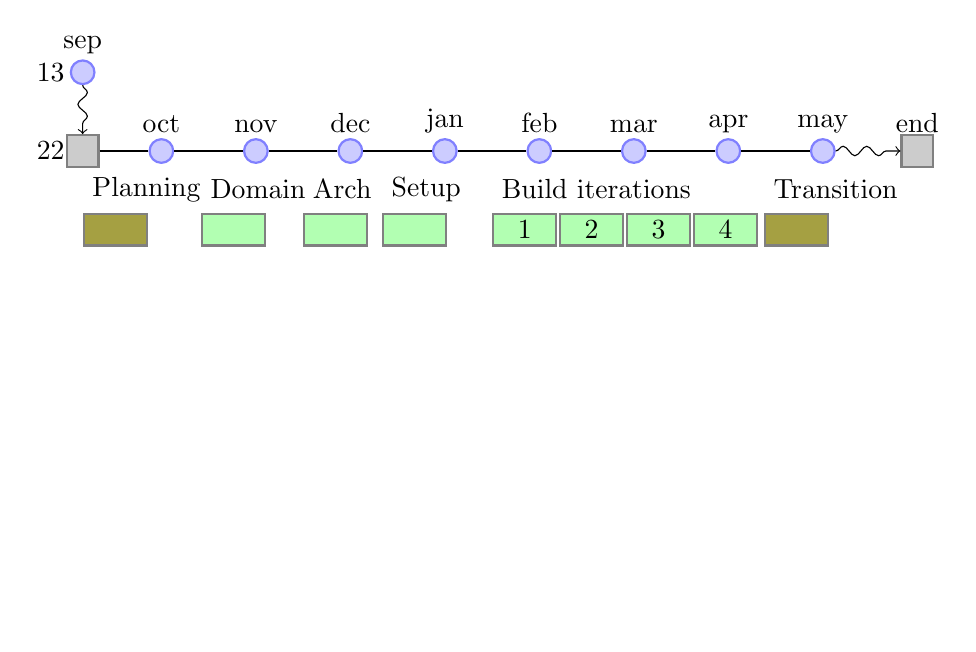
\begin{tikzpicture}
 	[month/.style={circle,draw=blue!50,fill=blue!20,thick,inner sep=0pt,minimum size=3mm},
	transition/.style={rectangle,draw=black!50,fill=black!20,thick,inner sep=0pt,minimum size=4mm},
	iteration/.style={rectangle,draw=black!50,fill=green!30,anchor=west,thick,inner sep=0pt,minimum height=4mm, minimum width=8mm},
	orgiter/.style={rectangle,draw=black!50,fill=yellow!60!black,anchor=west,thick,inner sep=0pt,minimum height=4mm, minimum width=8mm}]
%%	[fill=green!70!blue,every path/.style={draw}]
	\newcounter{ysize};
	\setcounter{ysize}{7};
	\newcommand{\y}{\value{ysize}}
	\node (sep) at (0,\y)    [month] {};
	\node (start) at (0,\y-1) [transition] {};
	\node (oct) at (1.0,\y-1)  [month] {};
	\node (nov) at (2.2,\y-1)    [month] {};
	\node (dec) at (3.4,\y-1)  [month] {};
	\node (jan) at (4.6,\y-1)    [month] {};
	\node (feb) at (5.8,\y-1)  [month] {};
	\node (mar) at (7.0,\y-1)    [month] {};
	\node (apr) at (8.2,\y-1) [month] {};
	\node (may) at (9.4,\y-1)   [month] {};
	\node (end) at (10.6,\y-1)   [transition] {};
	\path (0,0);
	\node (planning) at (0, \y-2) [orgiter] {};
	\node [above=3mm of planning.north west,anchor=west] {Planning};
	\node (domain) at (1.5, \y-2) [iteration] {};
	\node [above=3mm of domain.north west,anchor=west] {Domain};
	\node (arch) at (2.8, \y-2) [iteration] {};
	\node [above=3mm of arch.north west,anchor=west] {Arch};
	\node (setup) at (3.8, \y-2) [iteration] {};
	\node [above=3mm of setup.north west,anchor=west] {Setup};
	\node (iterA) at (5.2, \y-2) [iteration] {1};
	\node [above=3mm of iterA.north west,anchor=west] {Build iterations};
	\node (iterB) at (6.05, \y-2) [iteration] {2};
	\node (iterC) at (6.9, \y-2) [iteration] {3};
	\node (iterD) at (7.75, \y-2) [iteration] {4};
	\node (transition) at (8.65,\y-2) [orgiter] {}; 
	\node [above=3mm of transition.north west,anchor=west] {Transition};
	\draw (sep) node[above=3pt] {sep};
	\draw (sep) node[left=3pt] {13};
	\draw (start) node[left=3pt] {22};
	\draw (oct) node[above=3pt] {oct};
	\draw (nov) node[above=3pt] {nov};
	\draw (dec) node[above=3pt] {dec};
	\draw (jan) node[above=3pt] {jan};
	\draw (feb) node[above=3pt] {feb};
	\draw (mar) node[above=3pt] {mar};
	\draw (apr) node[above=3pt] {apr};
	\draw (may) node[above=3pt] {may};
	\draw (end) node[above=3pt] {end};
	\draw (start) -- (oct) -- (nov) -- (dec) -- (jan) -- (feb) -- (mar) -- (apr) -- (may);
	\draw [->,decorate,decoration={snake,amplitude=.6mm,segment length=3mm,post length=1mm}] (sep) -- (start);
	\draw [->,decorate,decoration={snake,amplitude=.6mm,segment length=3mm,post length=1mm}] (may) -- (end);
%	\path [fill] (-.2, \y-2) rectangle (2, \y-1.75);
	

%    % draw vertical lines
%    \foreach \x in {0,1,2,4,5,7}
%      \draw (\x cm,3pt) -- (\x cm,-3pt);

  \end{tikzpicture}
\end{frame}
  
\begin{frame}{Process Overview}
	\begin{columns}
		\begin{column}[t]{5cm}
			{\bf Process}
			\begin{itemize}
				\item <1->Planning phase: DAD approach (Disciplined Agile Delivery)
				\item <1->Domain analyses
				\item <1->Iteration 0 Architecture
				\item <1->Iteration 1 Build procedures and first prototype
				\item <1->iteration 2, 3, 4, 5 software development
				\item <1->\textit{Final Demo}$\leftarrow$
				\item <1->\textbf{transition}
			\end{itemize}
		\end{column}
		\begin{column}[t]{5cm}
			\textbf{Development factors}
			\begin{itemize}
				\item <2->Time boxing
				\item <2->Early switch to \qt
				\item <2->UI design : \qml
				\item <2->Qml / xmas integration: fat interface
				\item <2->Reorg OU $\rightarrow$ Communication drop
			\end{itemize}
		\end{column}
	\end{columns}
\end{frame}

\begin{frame}{Contribution to research project}
	\textbf{Contribution in different area's}
	\begin{itemize}
		\item {\bf Research support}
		\begin{itemize}
			\item papers to reason about verification tools of \Noc
			\item developers and testers of verification tools
			\item marketing of research efforts at OU and Radboud university
		\end{itemize}
		\item {\bf Design support}
		\begin{itemize}
			\item design and verification of new \Noc
		\end{itemize}
	\end{itemize}

\end{frame}

\begin{frame}{Example NoC}

\end{frame}

%% Demo XMAS Designer
\begin{frame}{Demo ``xmd'' \underline{x}MAS \underline{m}odel \underline{d}esigner}

	\begin{columns}
		\begin{column}[b]{0.8\textwidth}
			\begin{itemize}
				\item built with Qt Quick2 technology
				\item easy and powerful QML JavaScript GUI language
				\item c++ logic interfacing
				\item signal-slot event handling
				\item platform independent
			\end{itemize}			
		\end{column}
		\begin{column}[c]{.5\textwidth}
			
\includegraphics[width=0.75\linewidth]{pictures/2a-xmd}
		\end{column}
	\end{columns}
		
\end{frame}

\begin{frame}{xmd - main application window}
	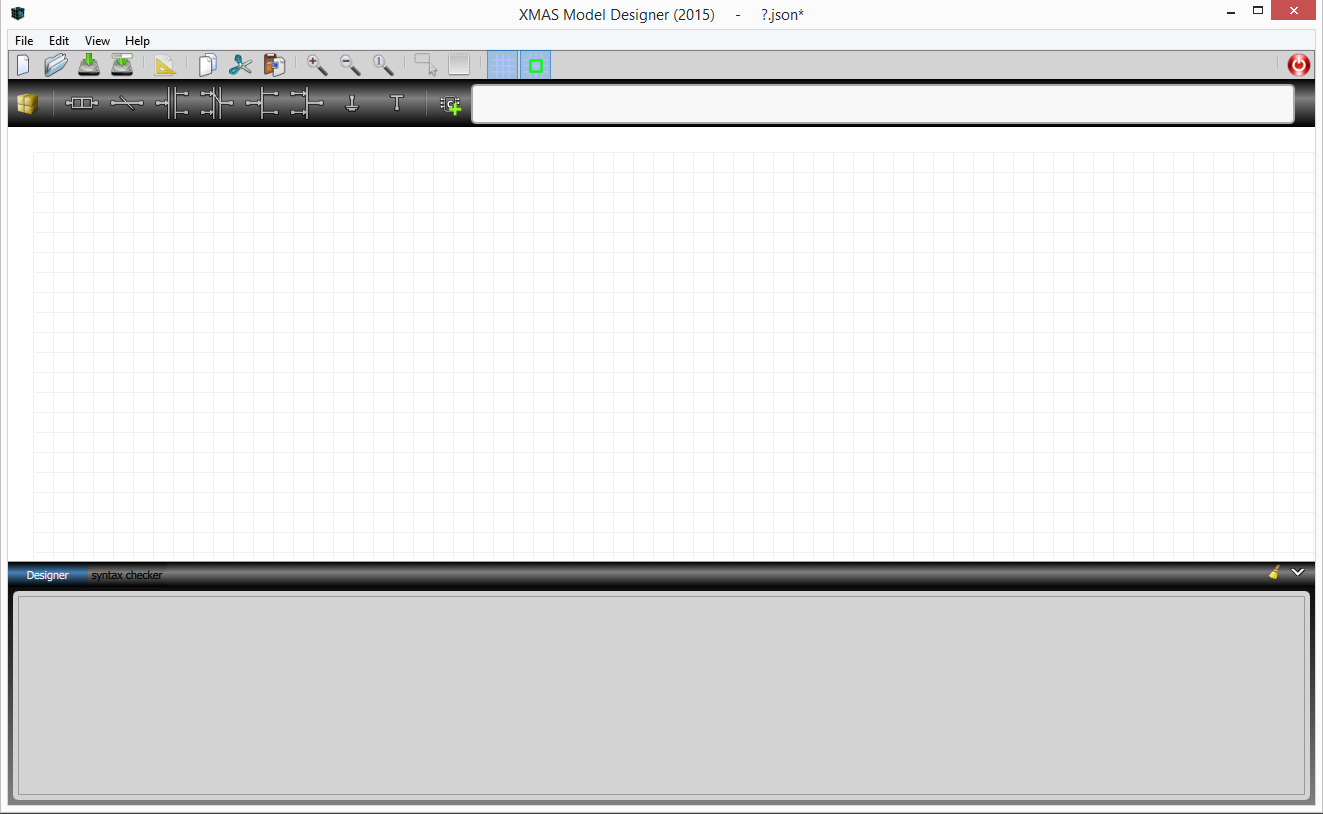
\includegraphics[width=.90\linewidth]{pictures/2b-xmd-empty}
\end{frame}
\begin{frame}{xmd - application setup}
	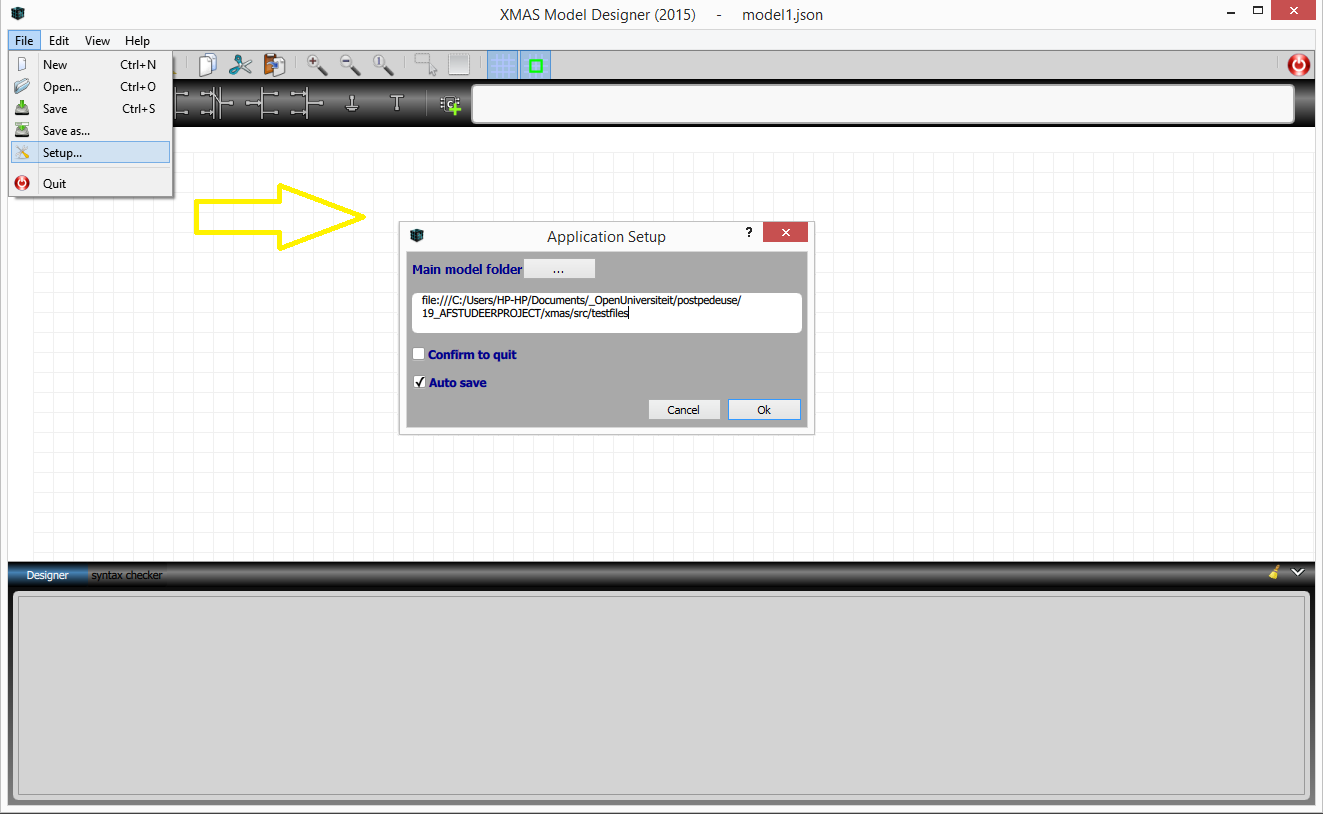
\includegraphics[width=.90\linewidth]{pictures/2c-xmd-app-setup}
\end{frame}
\begin{frame}{xmd - model setup}
	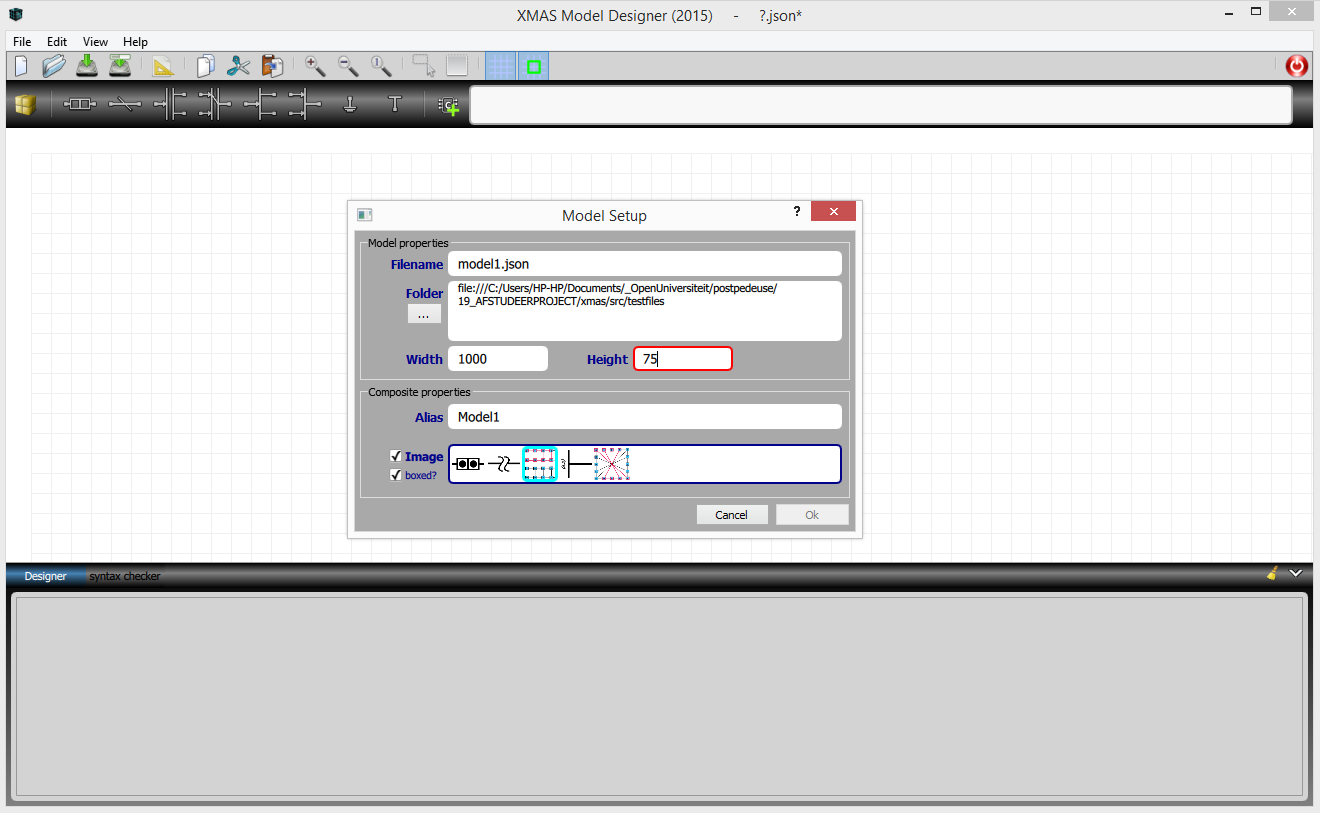
\includegraphics[width=.90\linewidth]{pictures/2d-xmd-model-setup}
\end{frame}
\begin{frame}{xmd - canvas}
	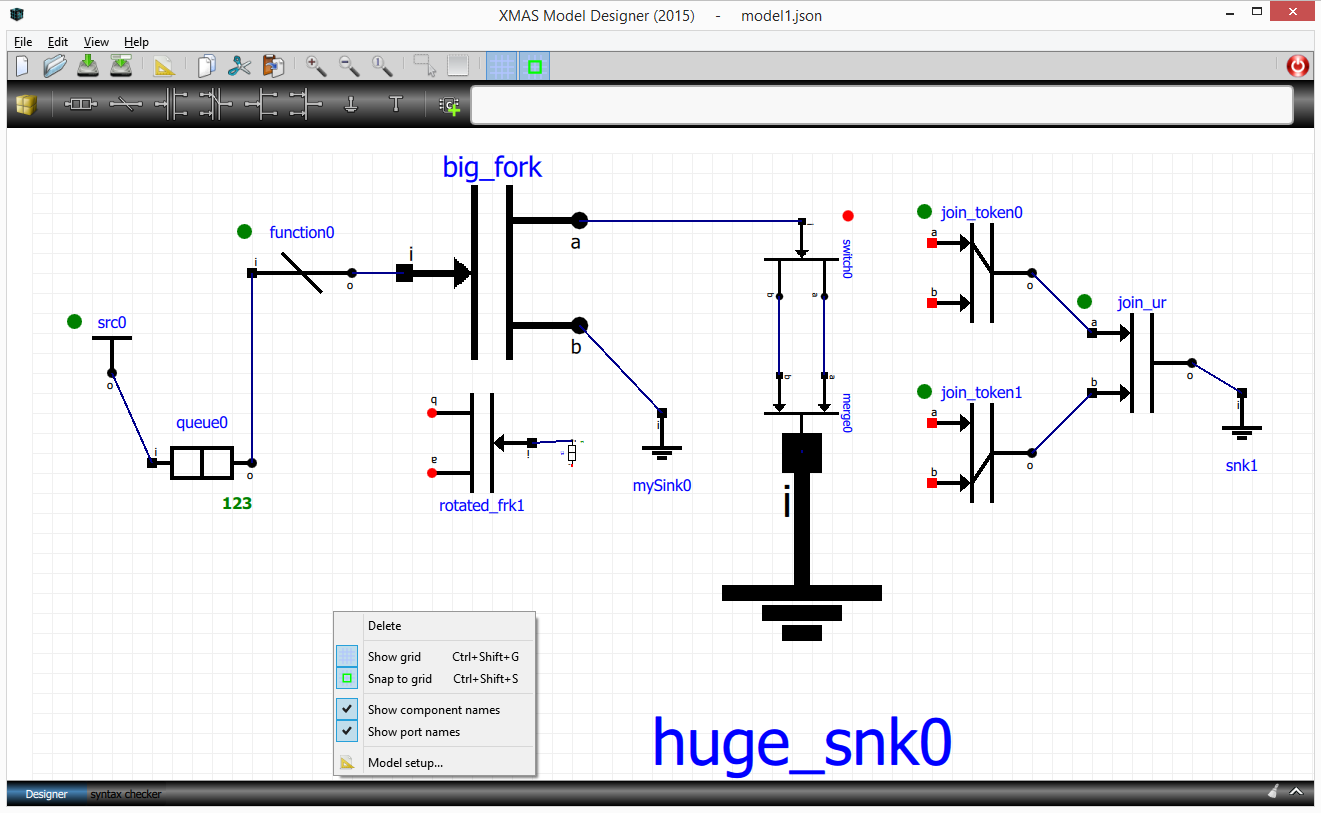
\includegraphics[width=.90\linewidth]{pictures/2e-xmd-canvas}
\end{frame}
\begin{frame}{xmd - group select}
	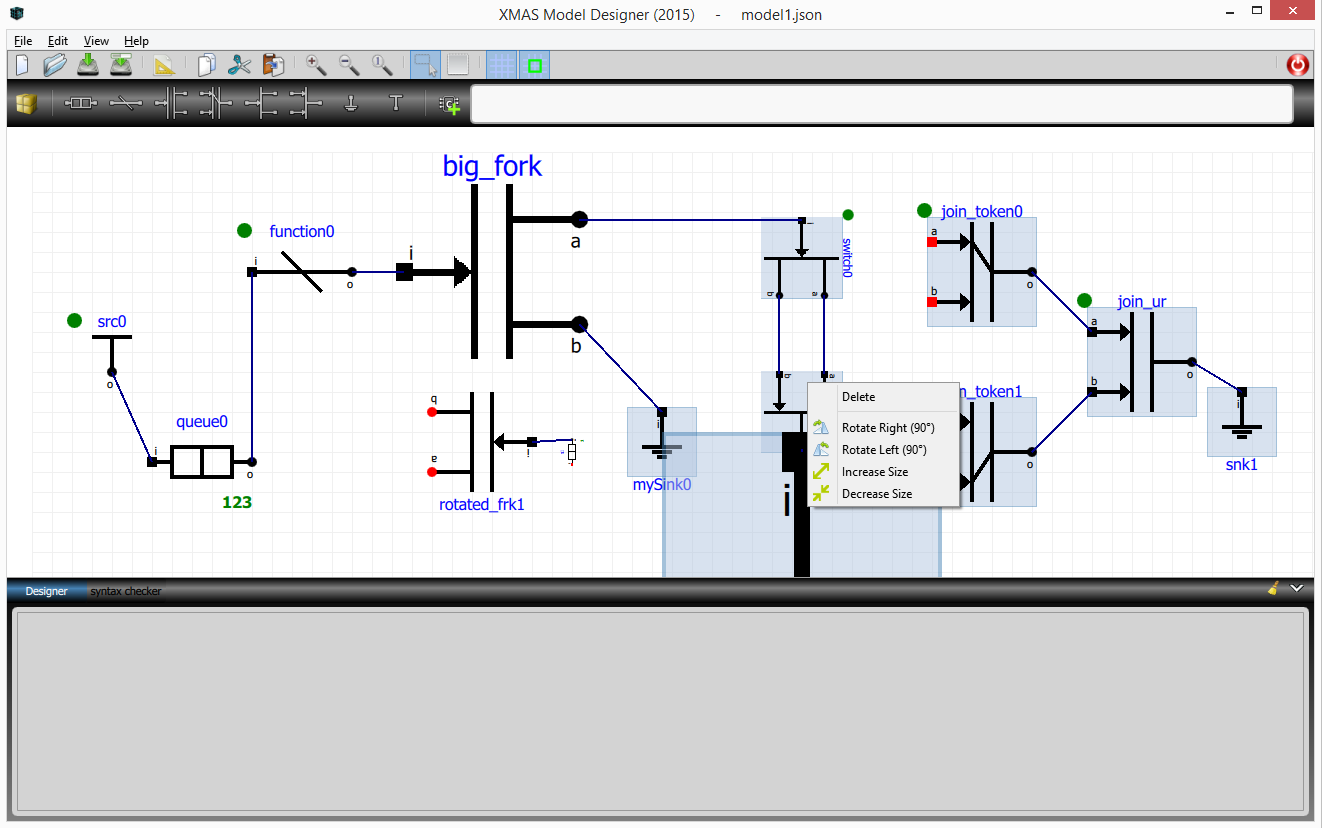
\includegraphics[width=.90\linewidth]{pictures/2f-xmd-canvas-groupselect}
\end{frame}
\begin{frame}{xmd - group delete}
	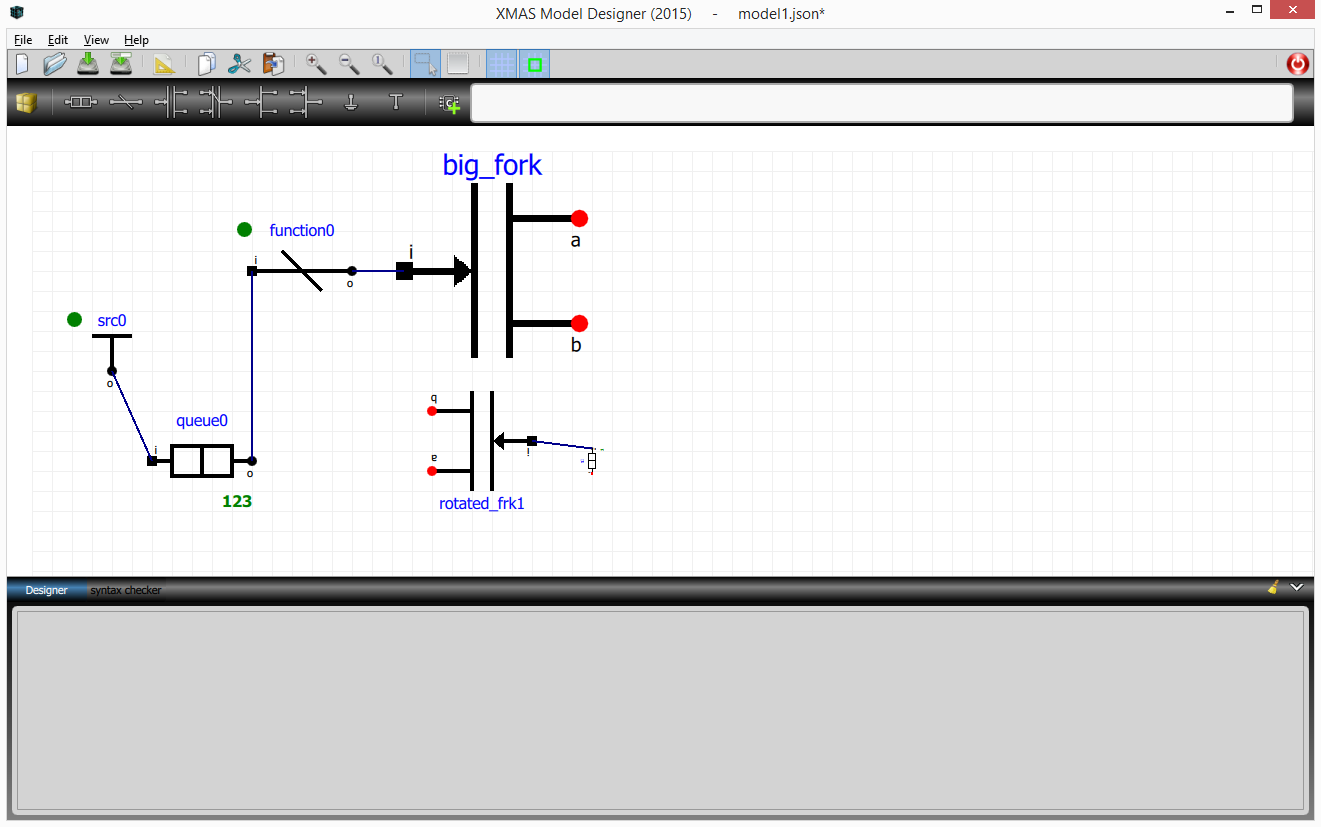
\includegraphics[width=.90\linewidth]{pictures/2g-xmd-canvas-delete}
\end{frame}
\begin{frame}{xmd - expression error feedback}
	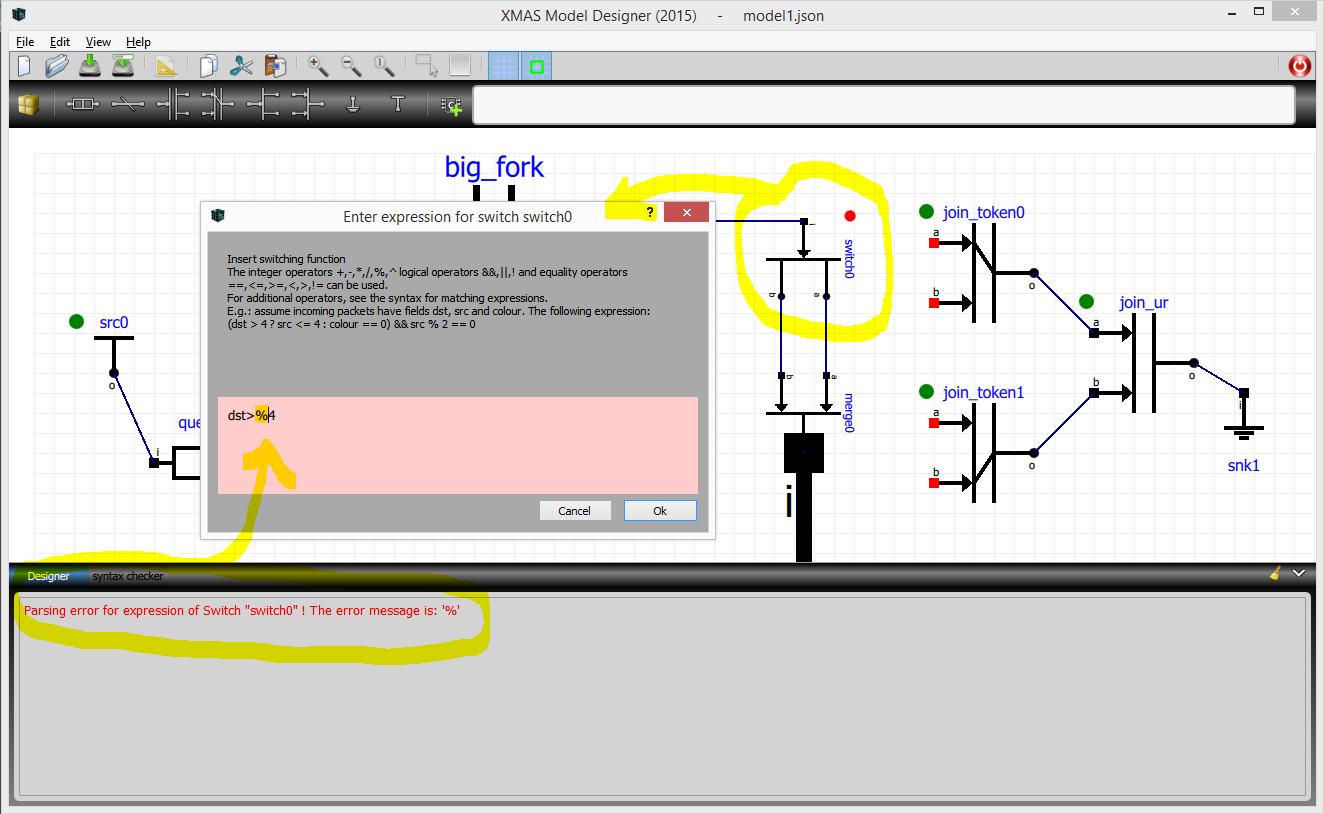
\includegraphics[width=.90\linewidth]{pictures/2h-xmd-expressiondialog-error}
\end{frame}
\begin{frame}{xmd - expression valid feedback}
	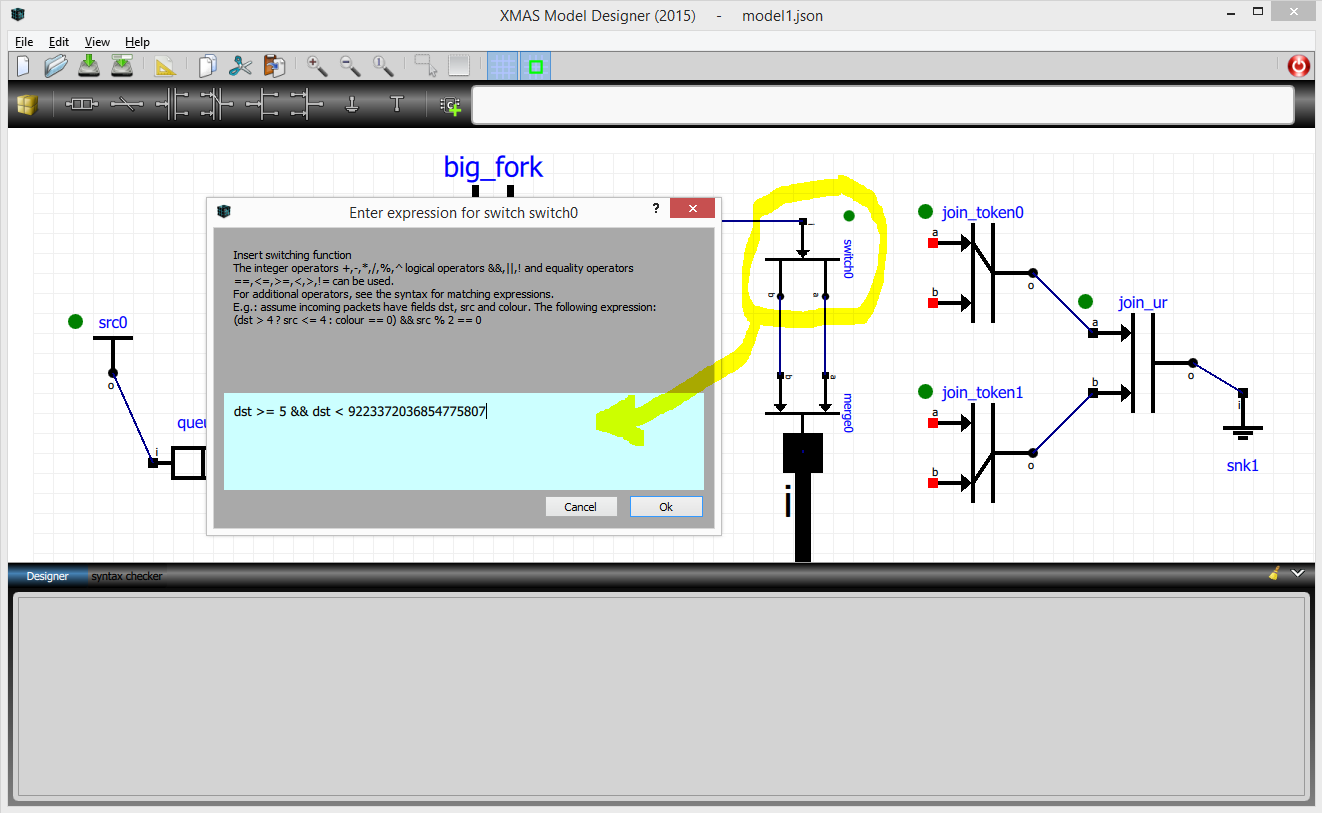
\includegraphics[width=.90\linewidth]{pictures/2i-xmd-expressiondialog-valid}
\end{frame}
\begin{frame}{xmd - composite library ``add''}
	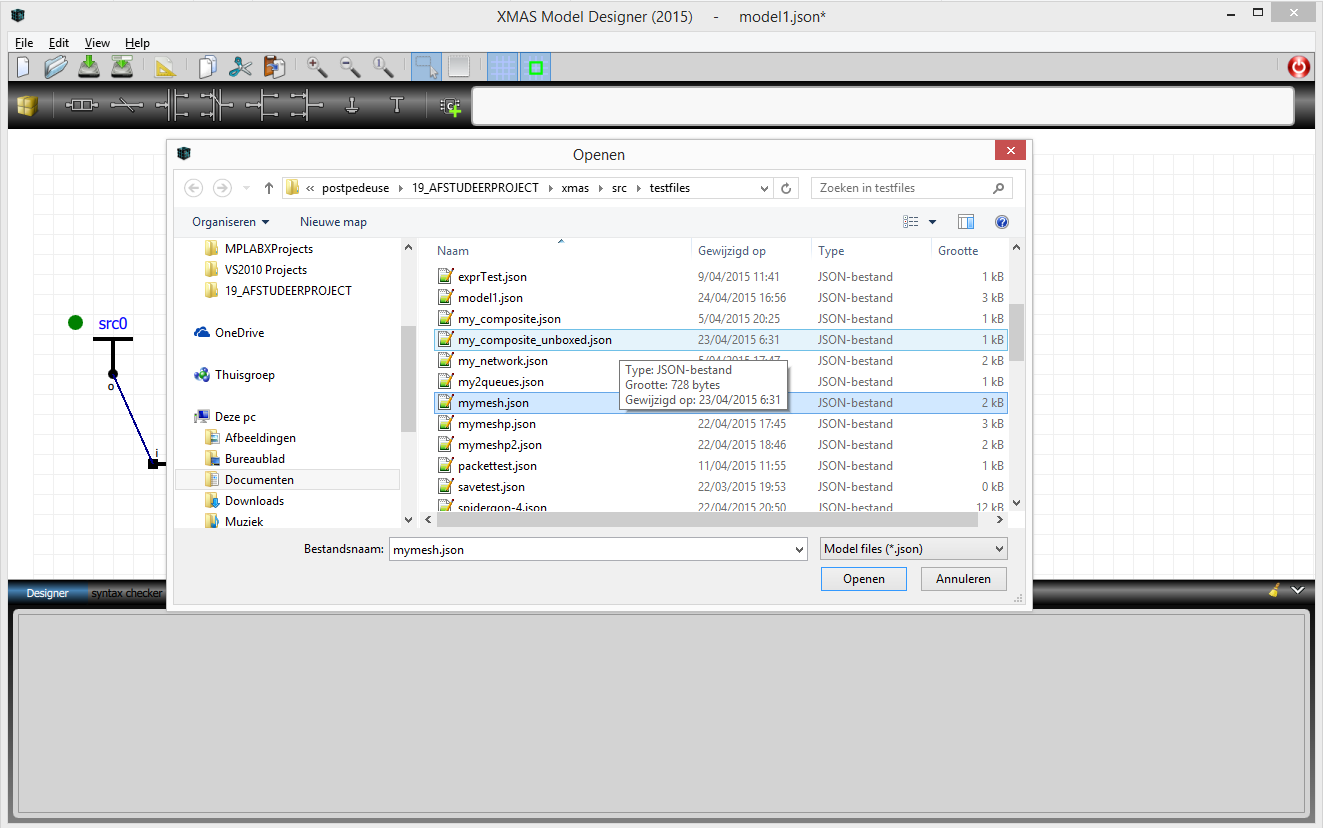
\includegraphics[width=.90\linewidth]{pictures/2j-xmd-compositelibrary-add}
\end{frame}
\begin{frame}{xmd - composite library ``remove''}
	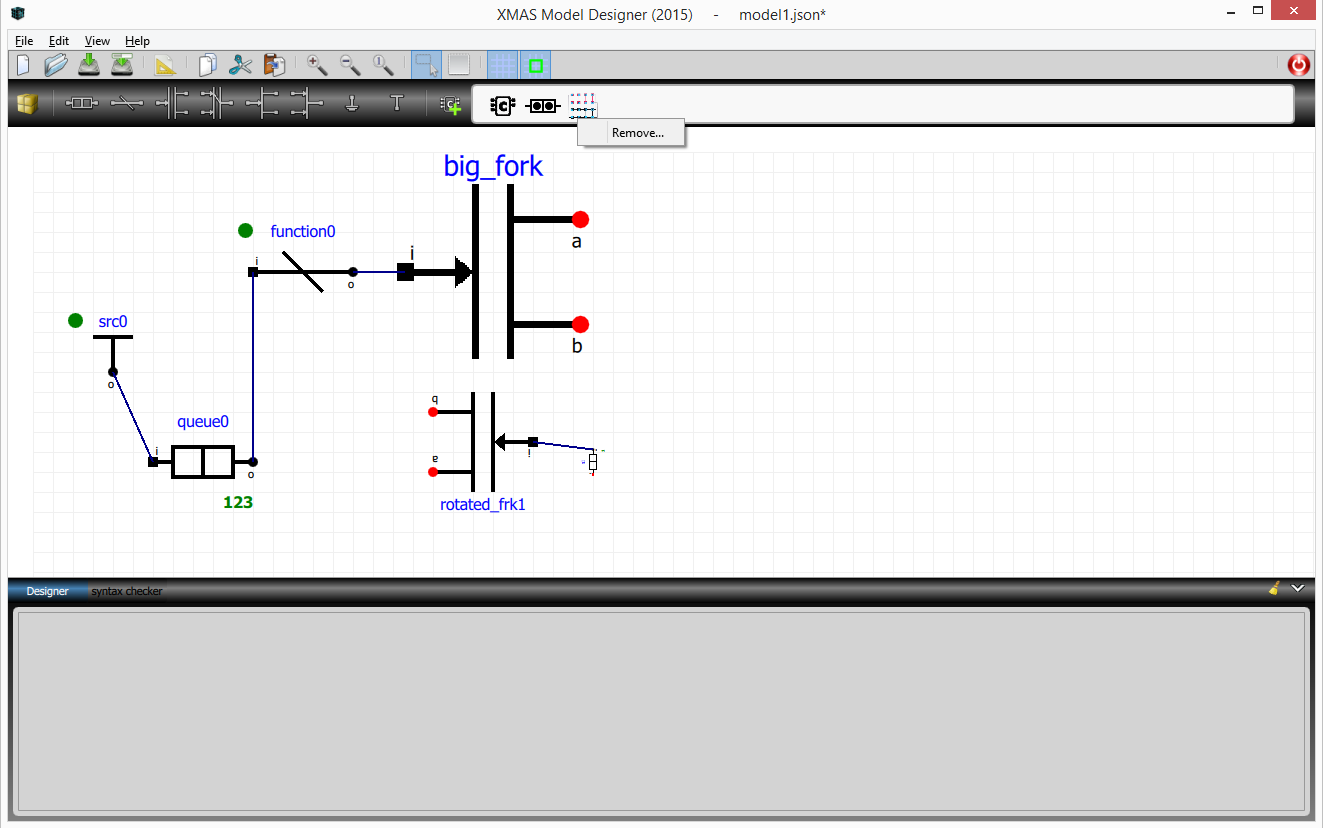
\includegraphics[width=.90\linewidth]{pictures/2k-xmd-compositelibrary-remove}
\end{frame}
\begin{frame}{xmd - composite use}
	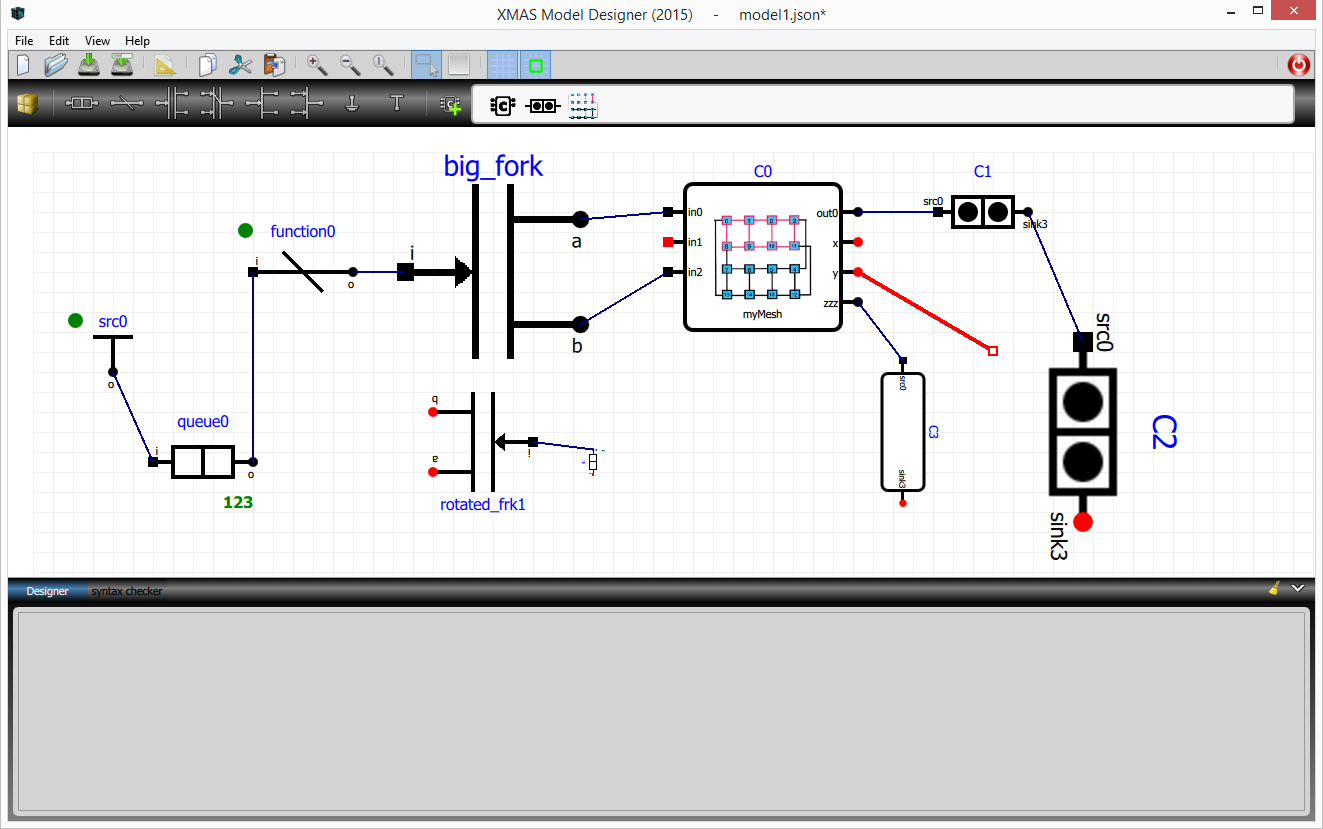
\includegraphics[width=.90\linewidth]{pictures/2l-xmd-composite-use}
\end{frame}
\begin{frame}{xmd - plug in}
	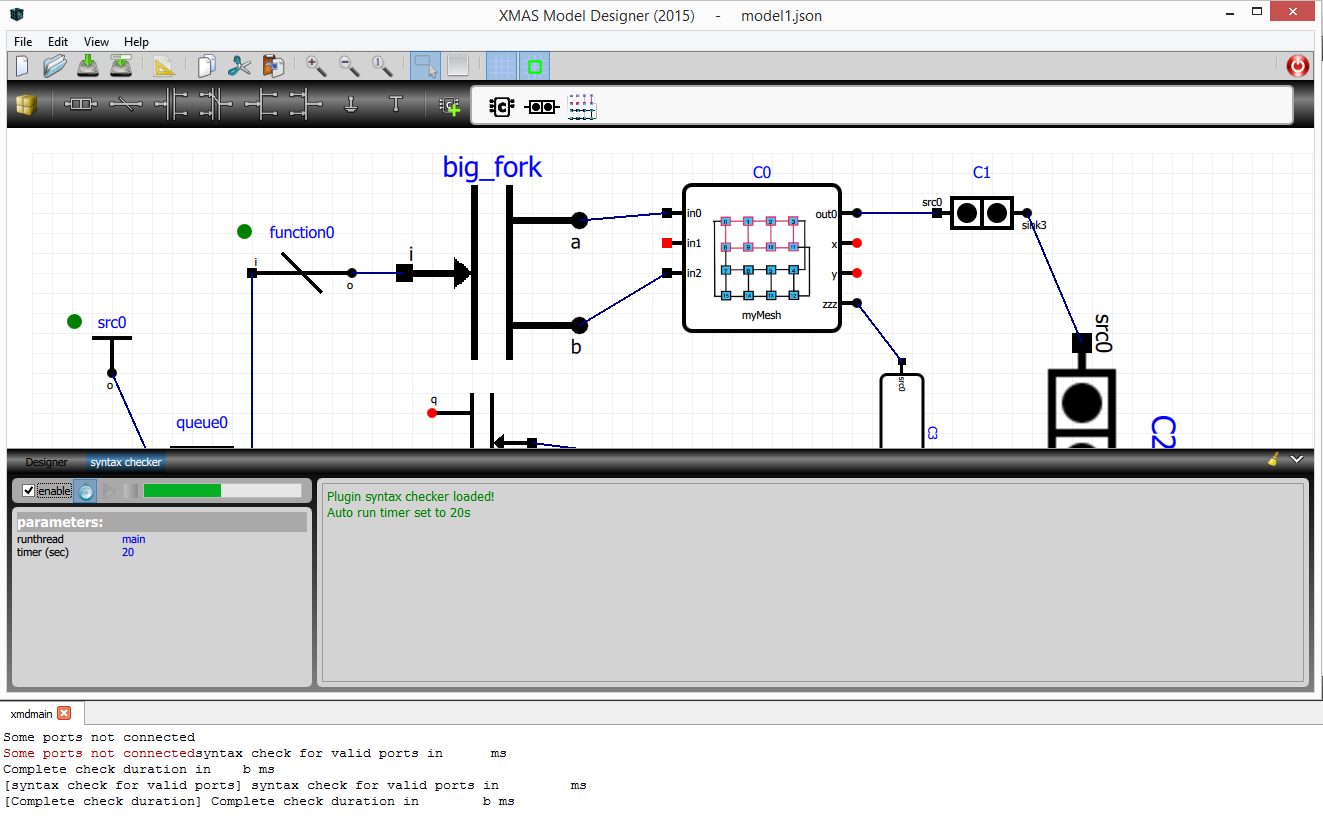
\includegraphics[width=.90\linewidth]{pictures/2m-xmd-plug-in}
\end{frame}
%% Demo XMAS Designer (end)



\begin{frame}{Specification model Data Layer iteration 1}

	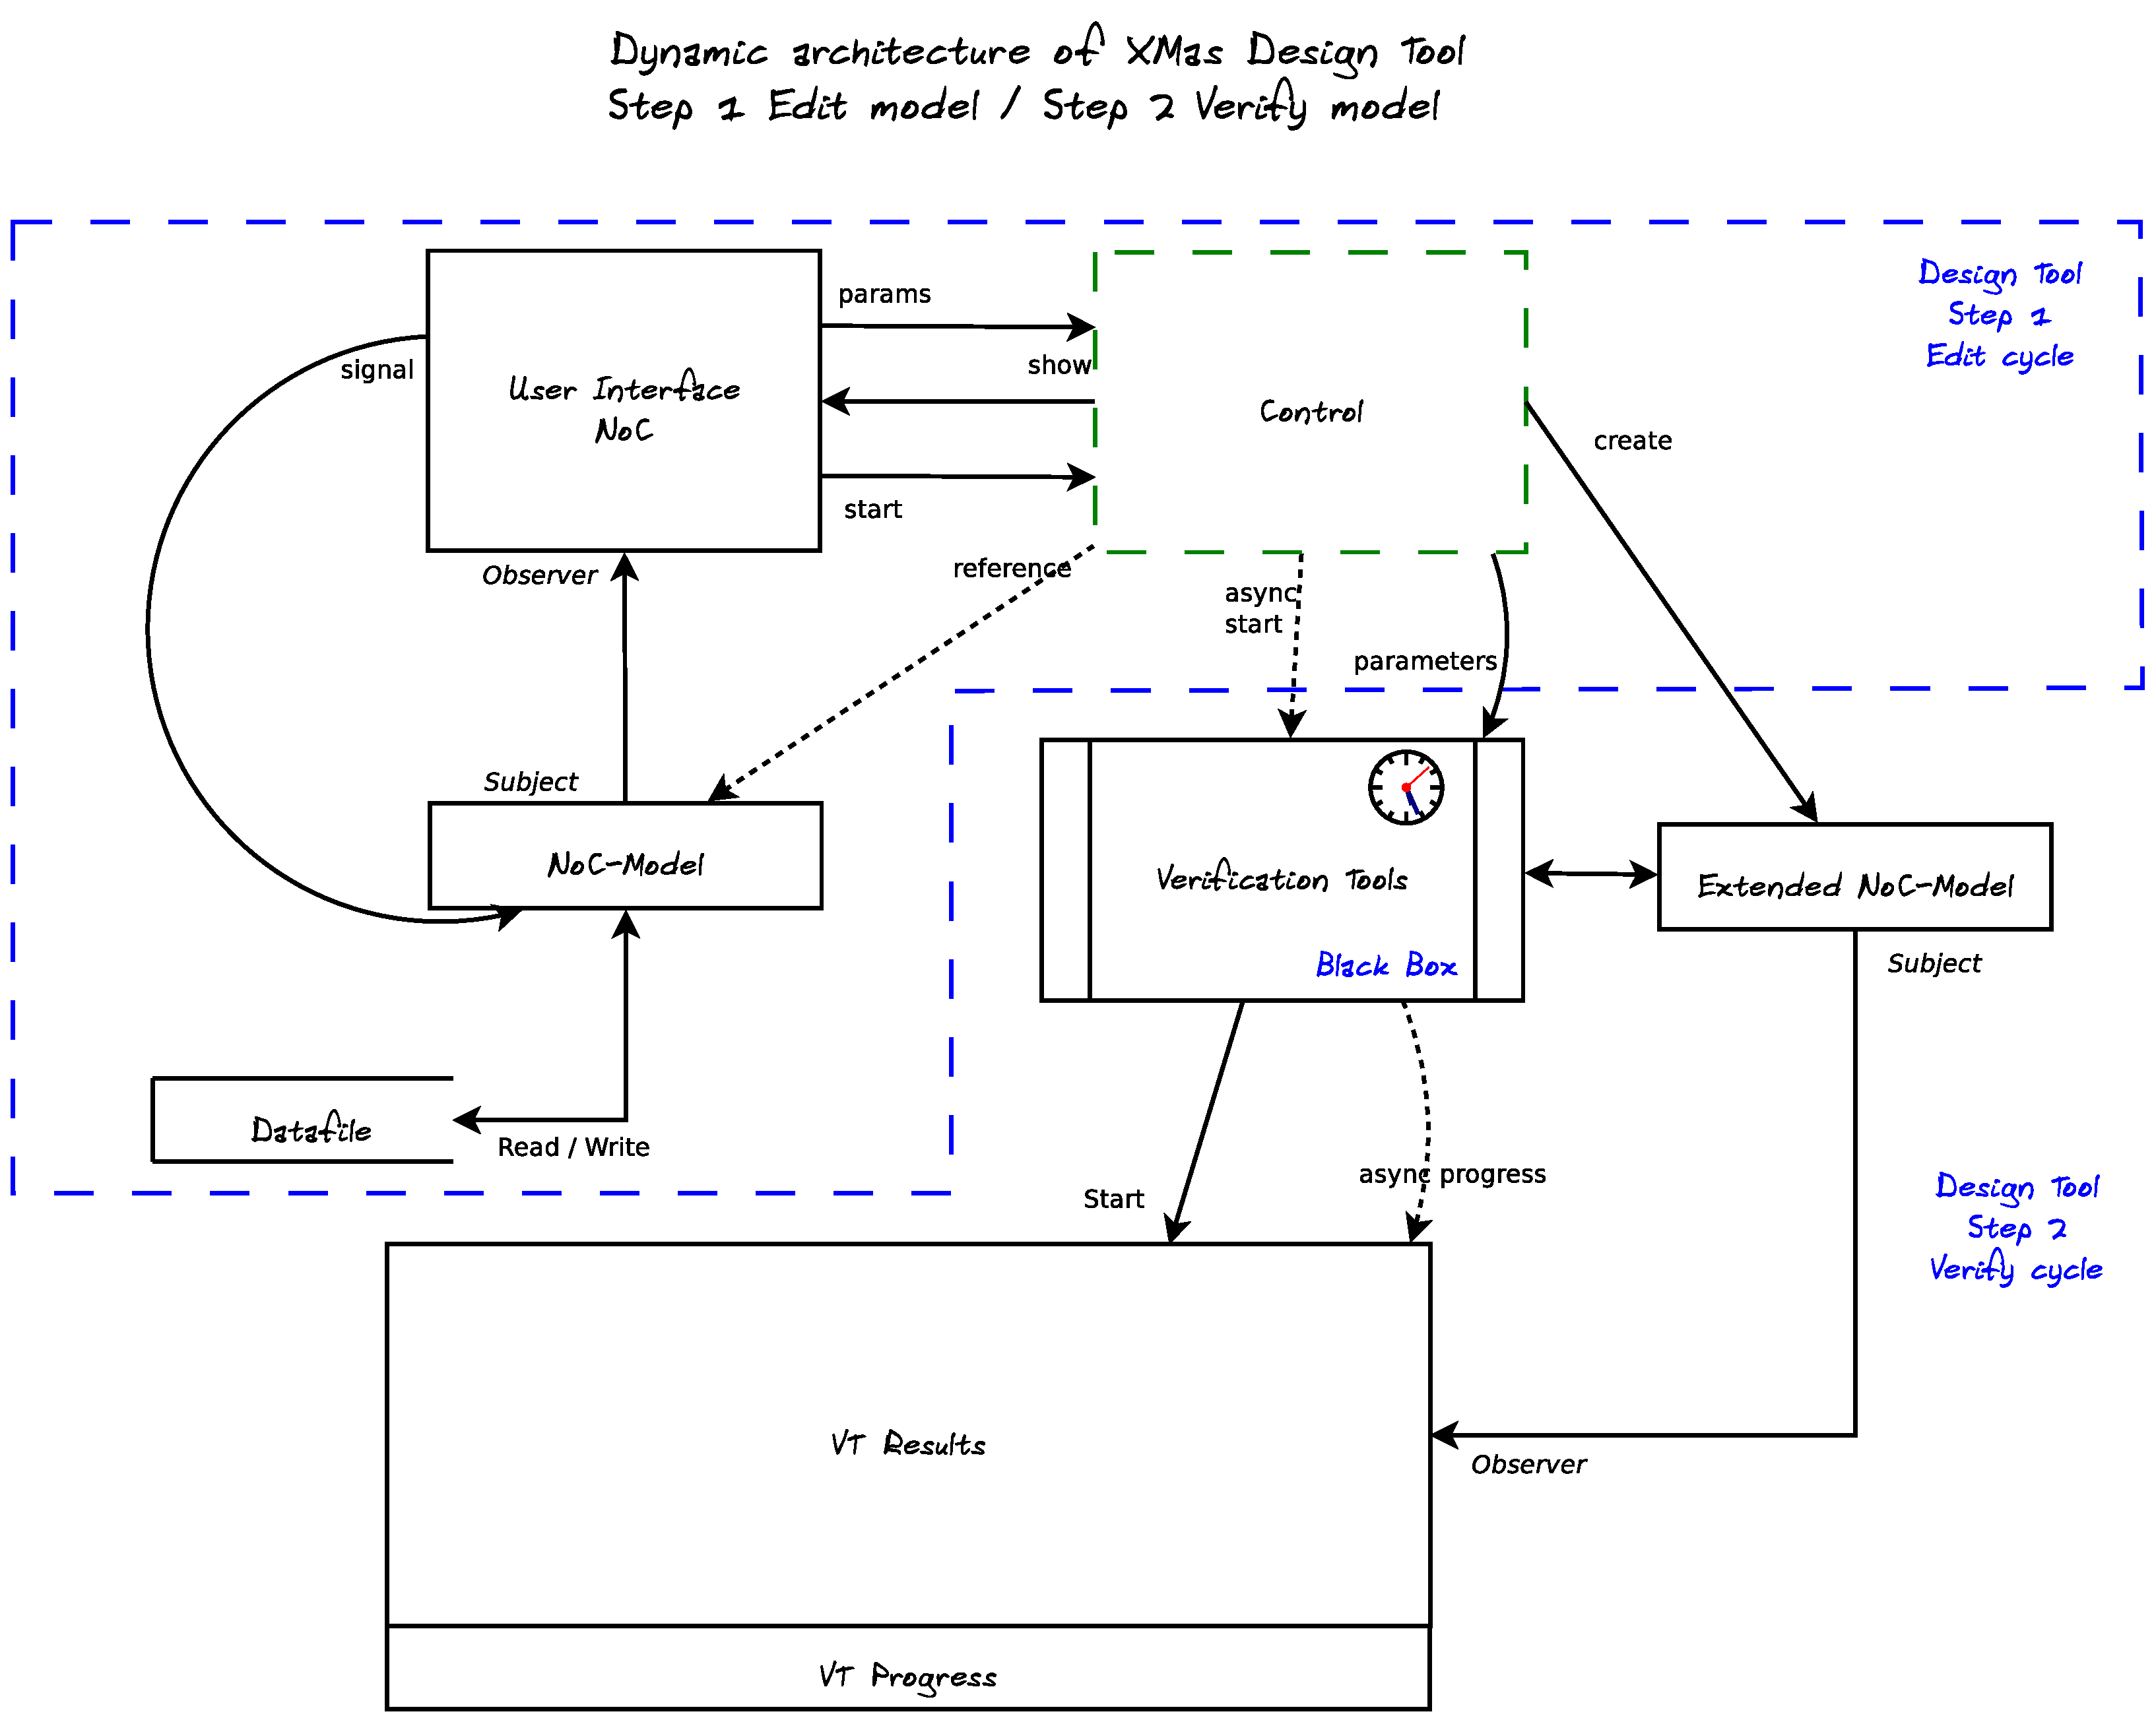
\includegraphics[width=.80\linewidth]{pictures/1c-architecture-dynamic-1}

\end{frame}

\begin{frame}{Implementation Data layer}

	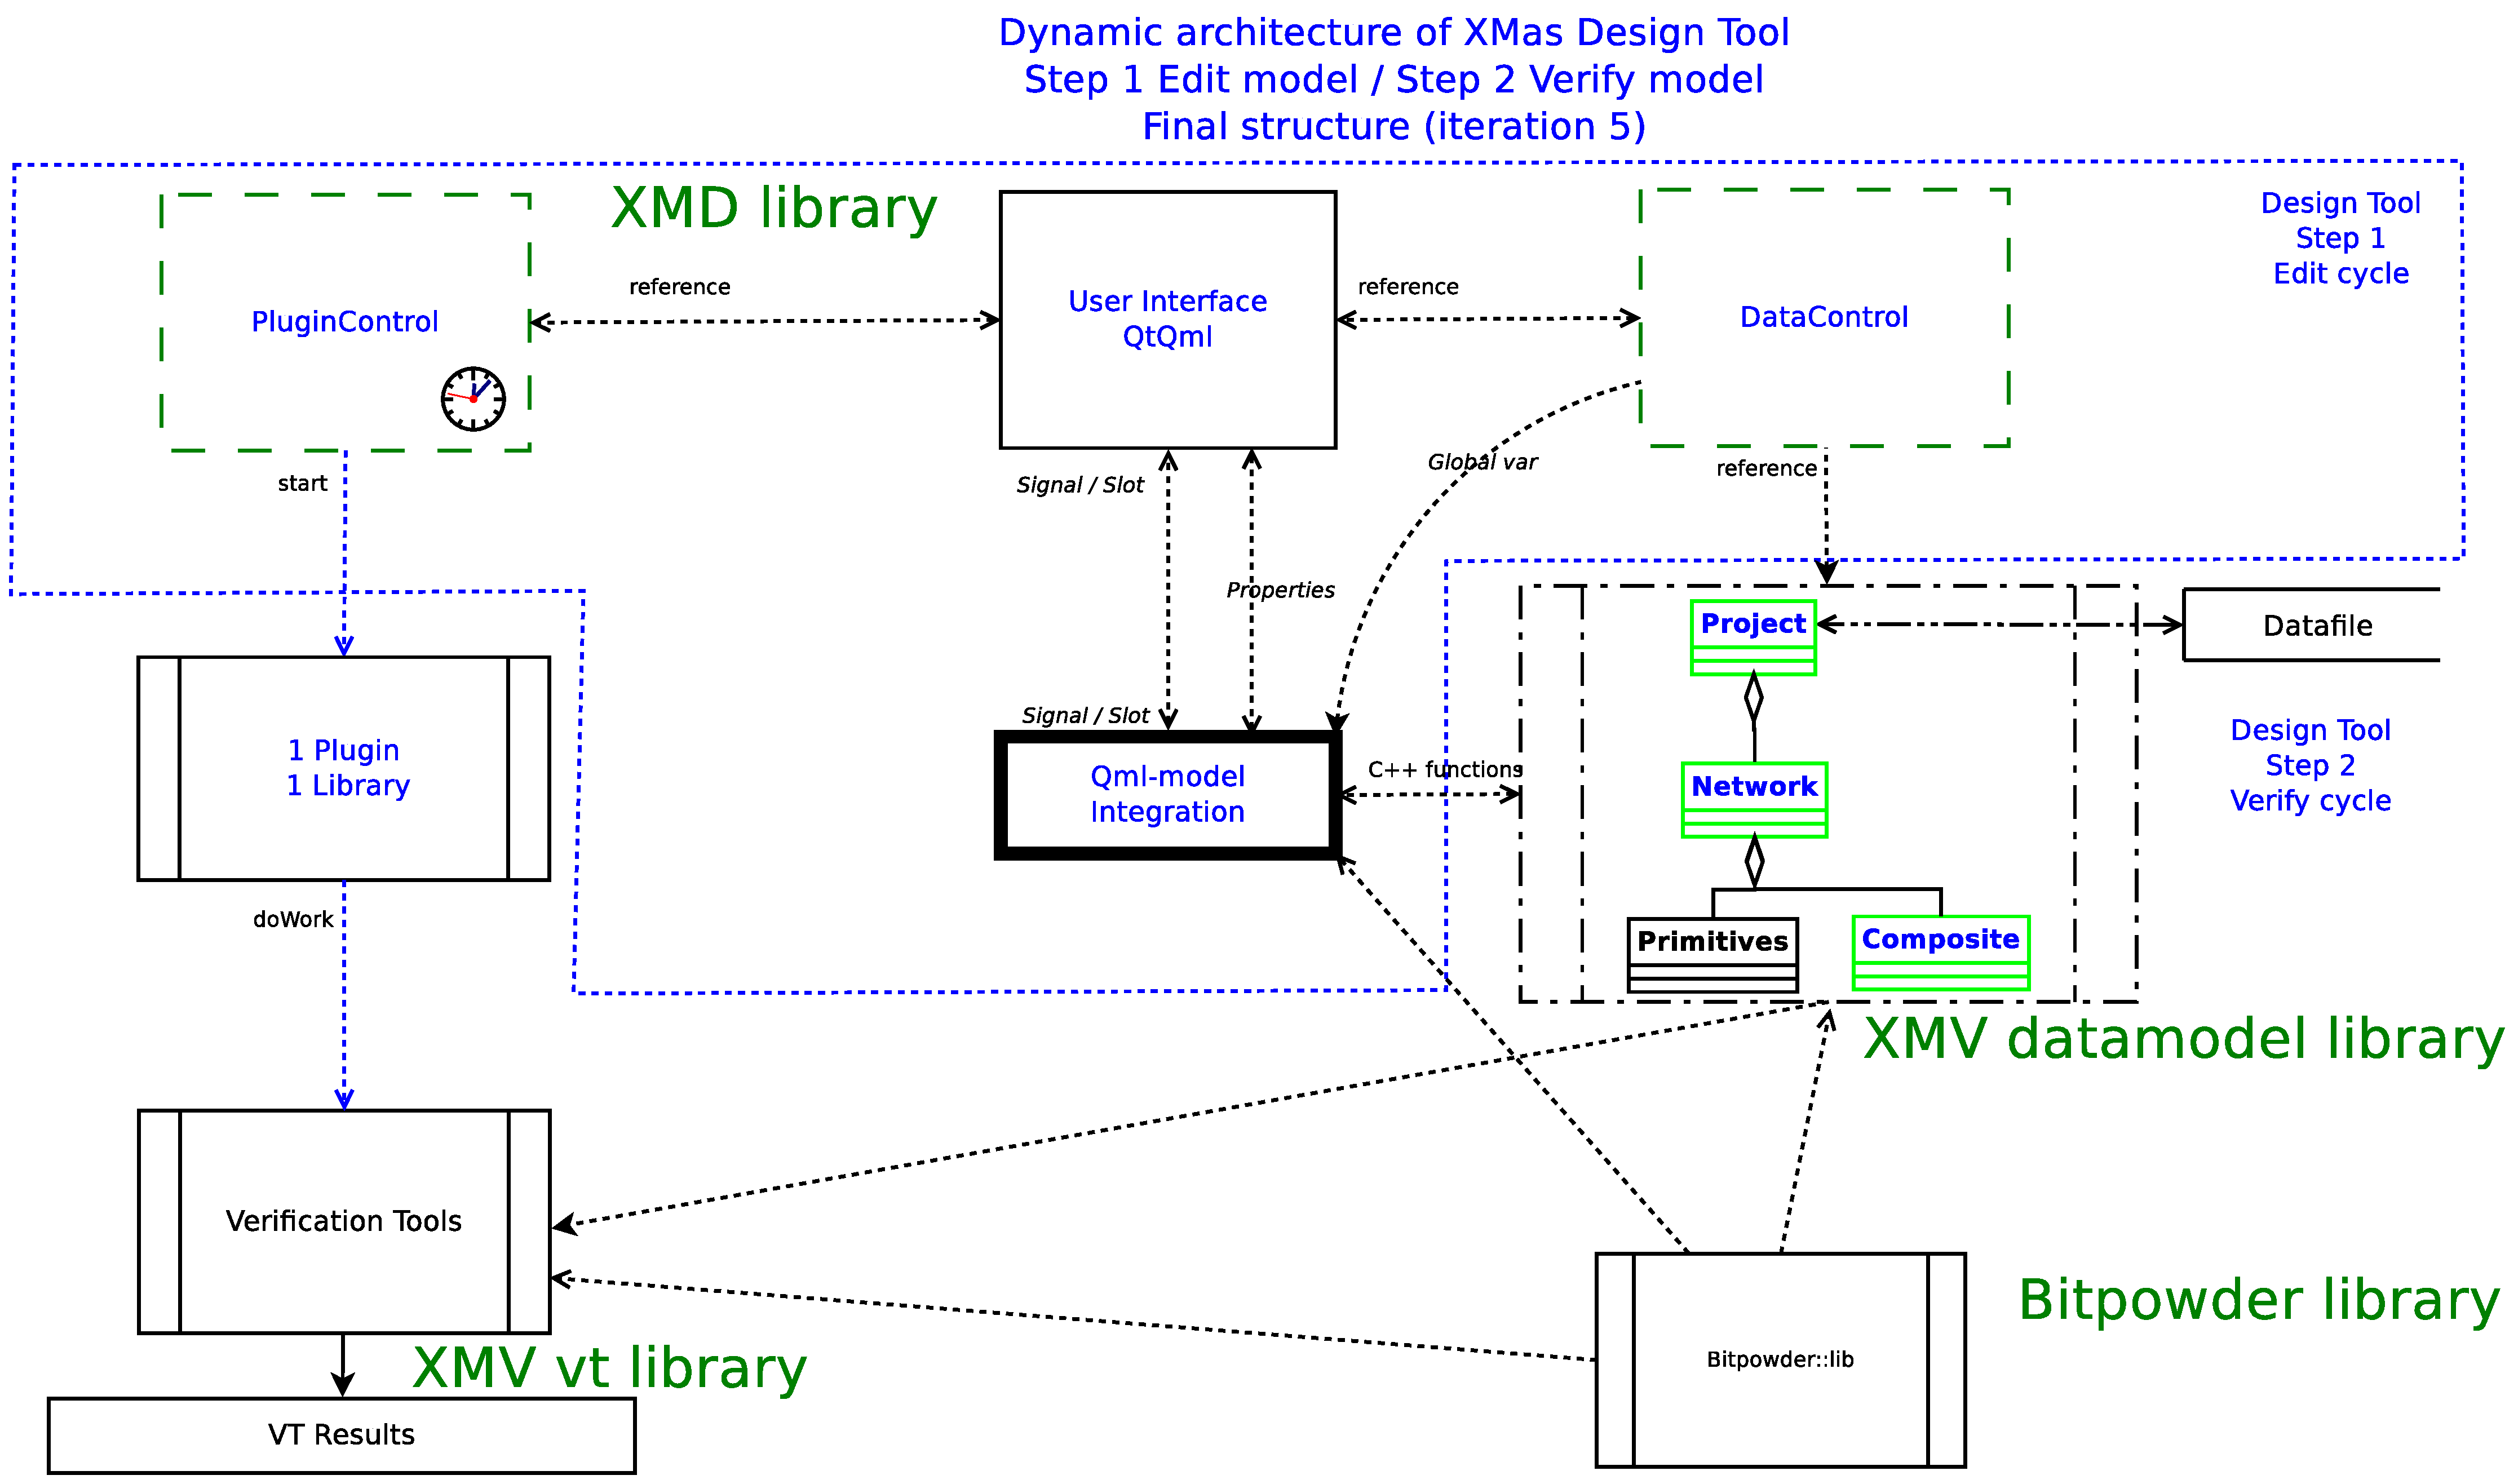
\includegraphics[width=.90\linewidth]{pictures/1c-architecture-dynamic-2}

\end{frame}

\begin{frame}{Process Reflection}
	\begin{itemize}
		\item {\bf Agile} 
				\begin{itemize}
					\item tools: skype: teamviewer, github, agilefant. Worked well.
					\item Internal communication: worked very well
					\item External communication: limited due to OU reorganisation
				\end{itemize}
		\item {\bf Planning}
				\begin{itemize}
					\item scheduling \& iterations: followed to a t.
					\item Influence OU reorg: risks increased
				\end{itemize}
		\item {\bf Design} 
			\begin{itemize}
				\item Switching to \qt				 (would do it again)
				\item Switching to \qml				 (would do it again)
				\item Switching to tight xmas integration (underestimated consequences)
			\end{itemize}
	\end{itemize}
\end{frame}

\begin{frame}{Product Reflection}
	\begin{itemize}
		\item {\bf User Interface} 
				\begin{itemize}
					\item Programming user interface in \qml worked out well.
							It was a lot easier than the conventional user interface
					\item Integration between user interface and data structures
							was painfull. For next time take more serious note
							of alternatives affecting coupling through an interface
					\item Composites finished ok. Was easier due to /qml
				\end{itemize}
		\item {\bf Data structures}
				\begin{itemize}
					\item Extensions (useful for visiting pattern) were a source
							of memory errors, that partly still existed when
							released. They are still being worked on.
					\item Composites: easy enough to create. It shows the way
							for parameterized objects.
					\item Getting parsing right was more difficult than we expected.
				\end{itemize}
	\end{itemize}
\end{frame}

\begin{frame}
	\begin{description}
		\item[Source code] github https://github.com/bvgastel (Nog te bepalen)
		\item[Documentation] github repo
	\end{description}
\end{frame}

\end{document}
